\section{An example: contact manager}

%Instead of listing all the features of Dart I thought about how to present them in a practical and more playful way. So I decided to introduce Dart by building a small contact manager.

%The interesting points of each listing will be explained afterwards. Thus most features of Dart will be explained in a practical way.

The contact manager will provide the following features:
\begin{itemize}
\item List all available contacts.
\item Add new contacts.
\end{itemize}

\subsection{Tools}

% Time to have a look on the available tools for developing with Dart.

Google provides some useful tools for developing with Dart.

First there is the Dart editor based on Eclipse\footnote{\url{http://www.eclipse.org/}} supporting syntax highlighting and autocompletion for Dart as shown in Figure \ref{figure:editor}.

\begin{figure}[h]
	\centering
  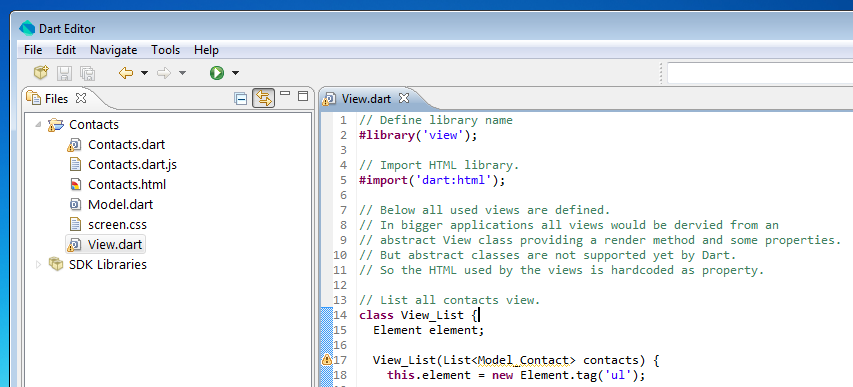
\includegraphics[width=0.8\textwidth]{images/editor.png}
	\caption{Dart editor with syntax highlighting}
	\label{figure:editor}
\end{figure}

For running Dart applications the code is translated to Javascript, so the application can be started in your default browser.

\begin{figure}[h]
	\centering
  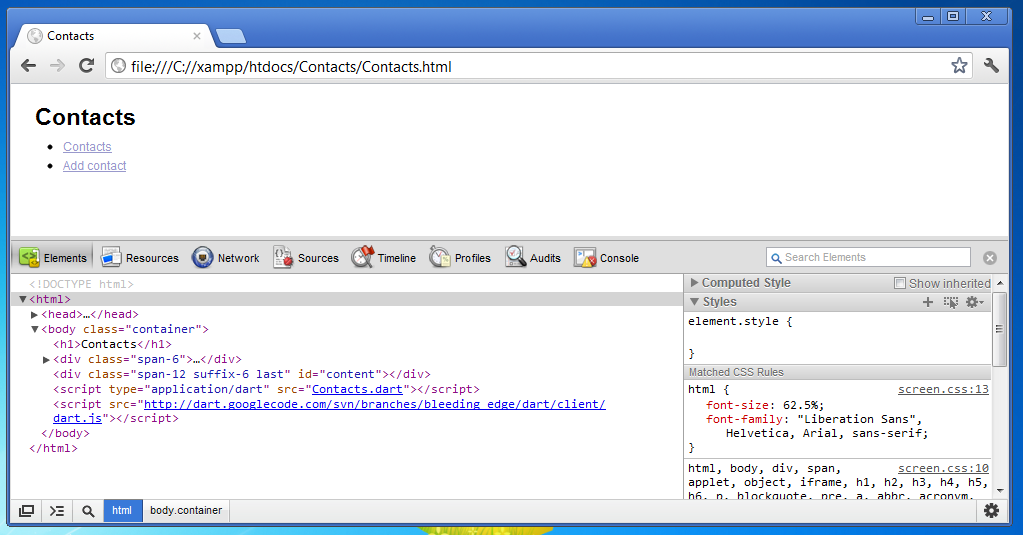
\includegraphics[width=0.8\textwidth]{images/dartium.png}
	\caption{Dartium}
	\label{figure:dartium}
\end{figure}

Dartium\footnote{\url{http://www.dartlang.org/dartium/index.html}} is a chromium-based browser -- see Figure \ref{figure:dartium} -- and provides the Dart VM. Using Dartium Dart applications can be run without compiling to Javascript.

% Similar to Chrome\footnote{\url{http://www.google.de/chrome}} Dartium includes the developer tools useful for debugging Dart code and investigating the DOM.

\subsection{Start}

% Create a new project using \emph{File} --- \emph{New application...} .
Listing \ref{listing:project-basic} shows the code automatically gernerated by the Dart editor after creating a new project:

\begin{lstlisting}[caption={Basic Dart program}\label{listing:project-basic}]
#import('dart:html');

class Contacts {

  Contacts() {
  }

  void run() {
    write("Hello World!");
  }

  void write(String message) {
    // the HTML library defines a global "document" variable
    document.query('#status').innerHTML = message;
  }
}

void main() {
  new Contacts().run();
}
\end{lstlisting}

\begin{itemize}
\item The Dart HTML library is imported using the \lstinline|import| keyword.% To see all built-in libraries use the Dart API reference\footnote{\url{http://api.dartlang.org/}}.
% \item The main application class -- ``Contacts'' -- is declared.% using the \lstinline|class| keyword.
\item \lstinline|write()| will append a given String to the DOM (Document Object Model\footnote{\url{http://en.wikipedia.org/wiki/Document_Object_Model}}) element with id ``status''. The method is optional typed by \lstinline|void|.
\item \lstinline|document.query('...')| searches a DOM element.
\item \lstinline|void main()| is the entry point of the script.
\end{itemize}

Figure \ref{figure:first-run} shows the output after running the application the first time.

\begin{figure}[htb]
	\centering
  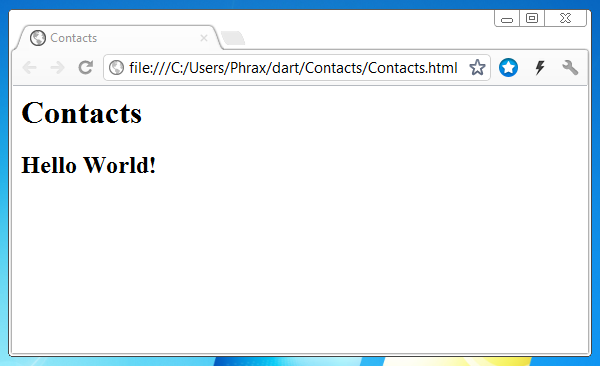
\includegraphics[width=0.9\textwidth]{images/first-run.png}
	\caption{First run of the application}
	\label{figure:first-run}
\end{figure}

\subsection{Modularity}
%\subsection{MVC}

%\begin{figure}[htb]
%	\centering
%  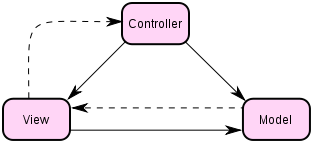
\includegraphics{images/mvc.png}
%	\caption{Model -- View -- Controller}
%	\label{figure:mvc}
%\end{figure}

%MVC\footnote{\url{http://de.wikipedia.org/wiki/Model_View_Controller}} (Model -- View -- Controller) is a popular design pattern used in class-based languages like Dart.

Although it is not necessarily needed, the application will be splitted up in multiple libraries according to the MVC (Model -- View -- Controller\footnote{\url{http://de.wikipedia.org/wiki/Model_View_Controller}}) design pattern.

For adding and querying all contacts the class \lstinline|Model| will provide \lstinline|add(Model_Contact contact)| and \lstinline|find_all()|. A single contact is represented by \lstinline|Model_Contact|.

\begin{lstlisting}[caption={Model}\label{listing:mvc-contact-model}]
// Define library name.
#library('model');

// On bigger applications an ORM system or similar would be used.
// For simplicity the Model class does only need to manage contacts.
class Model {
  
  static List<Model_Contact> contacts;
  
  // Add a new contact to the list.
  static void add(Model_Contact contact) {
    
  }
  
  // Returns a list of all contacts.
  // Currently the contacts are hard coded for simplicity.
  // They could also be loaded from a server via AJAX.
  static List<Model_Contact> find_all() {
    
  }
}

// Model for single contact.
class Model_Contact {}
\end{lstlisting}

\begin{itemize}
\item \lstinline|#library('model')| will define a new library named ``model''.
\item All contacts will be saved in  \lstinline|static List<Model_Contact> contacts|.
%\item A method for adding a new contact with no return value (\lstinline|void|) is declared.
%\item To retrieve the list of all contacts \lstinline|find_all()| can be used. It will return a list containing all contacts.
\end{itemize}

The class ``Contacts'' will be the controller. The actions for the navigation will be implemented as event handlers in the \lstinline|run()| method as seen in Listing \ref{listing:mvc-controller}.

\begin{lstlisting}[caption={Controller}\label{listing:mvc-controller}]
// Main application class with initialization and all needed actions.
class Contacts {

  Contacts() {
  }

  // Will do all the initialization
  // and set up all needed event handlers.
  void run() {
    // Event handler for adding a new contact.
    var add_handler = (Event event) {

    };

    // Event handler for listing all contacts.
    var list_handler = (Event event) {

    };
  }
}
\end{lstlisting}

\begin{itemize}
\item Functions can be assigned to variables -- both event handlers are assigned to the appropriate variables \lstinline|add_handler| and \lstinline|list_handler|.
\end{itemize}

The views are implemented as independant classes. They could also be derived from an abstract class ``View'' but for now Dart does not support abstract classes:

\begin{quotation}
``Dart will support abstract classes and abstract methods. As of 2012-04-04, abstract is not yet implemented.''\cite{LangTour}
\end{quotation}

Listing \ref{listing:mvc-view} shows the declarations of the views we will use  throughout the application. % They, too, will be kept in their own library.

\begin{lstlisting}[caption={Views}\label{listing:mvc-view}]
// Define library name
#library('view');

// Import HTML library.
#import('dart:html');

// The view used to list all contacts.
class View_List {
  // Constructor.
  Element element;

  View_List () {
    // Create HTML...
  }
}

// Add a new contact view.
class View_Add {
  Element element;

  // Constructor.
  View_Add () {
    // Create HTML...
  }
}
\end{lstlisting}

\begin{itemize}
\item \lstinline|#library('view')| defines the library for the views.
% \item Import Dart's HTML library.
\item The constructors of the views will build up the HTML.
\end{itemize}

\subsection{Contact model}

A contact will have the following attributes with the given types:

\begin{itemize}
\item ID -- \lstinline|num|.
\item First name -- \lstinline|String|.
\item Last name -- \lstinline|String|.
\item Phone number -- \lstinline|String|.
\item Email address -- \lstinline|String|.
\end{itemize}

Listing \ref{listing:model-1} shows the typed implementation of these attributes.

\begin{lstlisting}[caption={Class attributes}\label{listing:model-1}]
// Model for single contact.
class Model_Contact {
  
  // Attributes are automatically declared private
  // because of the prefixed underscore.
  num _id;
  String _first_name;
  String _last_name;
  String _phone;
  String _email;
}
\end{lstlisting}

\begin{itemize}
\item All attributes are declared private by prefixing the underscore -- making \lstinline|public| and \lstinline|private| keywords redundant.
% \item \lstinline|num| -- for all kinds of numeric values -- and \lstinline|String| are built-in types.
\end{itemize}

Dart is an optional typed language and supports multiple built-in types\footnote{\url{http://www.dartlang.org/language-tour/}}. To declare untyped variables the \lstinline|var| keyword can be used.

Because all attribtues in the model are declared as private we have to implement getters and setters to get access.

\begin{lstlisting}[caption={Getters and Setters}\label{listing:model-2}]
// Getters and setters for all attributes.
// Note the shorthand syntax used.
String get first_name() => this._first_name;
set first_name(String first_name) => this._first_name = first_name;
  
String get last_name() => this._last_name;
set last_name(String last_name) => this._last_name = last_name;
  
String get phone() => this._phone;
set phone(String phone) => this._phone = phone;
  
String get email() => this._email;
set email(String email) => this._email = email;
\end{lstlisting}

\begin{itemize}
\item Using the \lstinline|get| keyword getters can be declared.
\item The \lstinline|set| keyword is the equivalent for declaring setters.
\item In Dart all kind of methods can be declared using a shorthand syntax using \lstinline|=>|.
\end{itemize}

The attributes can now be accessed as if they were public attributes -- see Listing \ref{listing:model-3}.

\begin{lstlisting}[caption={Using getters and setters}\label{listing:model-3}]
// The attributes can be handled as if they were public.
contact.first_name = "David";
contact.last_name = "Stutz";
\end{lstlisting}

%\begin{itemize}
%\item Getters and setters declared using \lstinline|get| or \lstinline|set| allow to access the referenced attribute by overloaded operators. Note that for getting one of the values \lstinline|var first_name = contact.first_name()| is not valid.
%\end{itemize}

Another feature not necessarily known from other class-based languages: named constructors -- Listing \ref{listing:model-4}.% This concept allows having multiple constructors for a class, distinguishable by names, without having to use optional parameters or polymorphism.

\begin{lstlisting}[caption={Named constructors}\label{listing:model-4}]
// Creates a contact from an id and a map of values,
// A good example for named constructors.
Model_Contact.values(num id, Map<String, String> values) {
   this._id = id;
   this._first_name = values['first_name'];
   this._last_name = values['last_name'];
   this._phone = values['phone'];
   this._email = values['email'];
}
\end{lstlisting}

\begin{itemize}
\item \lstinline|Model_Contact.values(num id, Map<String, String> values)| declares the constructor named ``values''.
%\item For setting the contact's attributes a map mapping strings to strings is used.
\end{itemize}

Maps and lists are provided by Dart's collection framework -- similar to the Java Framework. Implementations of the collection framework can be found in the API reference\footnote{\url{http://api.dartlang.org/dart_core.html}}.

%Listing \ref{listing:model-5} shows the usage of the named constructor declared in listing \ref{listing:model-4} and another example for declaring maps.

%\begin{lstlisting}[caption={Using named constructors}\label{listing:model-5}]
%// The contacts values.
%Map<String, String> values = {
%  'first_name' : 'David',
%  'last_name' : 'Stutz',
%  'phone' : '0178 636 1771',
%  'email' : 'david.stutz@rwth-aachen.de',
%};
%// Create a new contact with id 1 and the given values.
%Model_Contact contact = new Model_Contact.values(1, values);
%\end{lstlisting}
%
%\begin{itemize}
%\item Maps can be declared using a comfortable JSON\footnote{\url{http://en.wikipedia.org/wiki/JSON}}-like syntax.
%\end{itemize}

\subsection{Views}

For DOM element creation -- Listing \ref{listing:view-2} -- there are named constructors provided. And manipulating DOM elements is simple:

\begin{lstlisting}[caption={DOM manipulation}\label{listing:view-2}]
// Creation by HTML:
Element element = new Element.html("<div>My element</div>");
// And by tag:
Element element = new Element.tag('div').innerHTML = "My element";
// Setting attributes:
element.attributes["readonly"] = true;
// Or classes:
element.classes.add('sidebar');
// Add further child elements:
element.nodes.add(new Element.html('<strong>Important!</strong>'));
// Remove all child elements:
element.nodes.clean();
\end{lstlisting}

\begin{itemize}
\item Element creation can be done using the shown named constructors -- by tag or by HTML.
\item Through \lstinline|attributes| and \lstinline|classes| the element's attributes and classes are accessible.
\item All child nodes of an element are -- similar to \lstinline|attributes| and \lstinline|classes| -- kept in a map allowing to remove nodes or add new ones.
\end{itemize}

\subsubsection{Adding a contact}

%The HTML markup should look like this:

%\begin{lstlisting}[language=HTML,caption={Form markup}\label{listing:view-2}]
%<table>
%  <tr>
%    <td><label for="first_name">First name</label></td>
%    <td><input type="text" name="first_name" /></td>
%  </tr>
%  <!-- Rows for the other attributes... -->
%  <tr>
%    <td colspan="2"><button type="submit">Submit</button></td>
%  </tr>
%</table>
%\end{lstlisting}
%
%\begin{itemize}
%\item Each row will represent a value of the contact containing a label and the corresponding input field.
%\item At the end a submit button is added.
%\end{itemize}

Let's create a form to add a new contact. Of course we could hard code the HTML, but Listing \ref{listing:view-3} shows another -- maybe more circumstantial -- way of creating the form.

\begin{lstlisting}[language=Java,caption={Form creation}\label{listing:view-3}]
// Add a new contact view.
class View_Add {
  
  Element element;
  
  View_Add() {
    this.element = new Element.tag('table');
    
    Map<String, String> rows = {
      'first_name': 'First name',
      'last_name': 'Last name',
      'phone': 'Phone',
      'email': 'E-Mail',
    };
    
    rows.forEach(function(key, value) {
      // Create the tr node.
      Element row = new Element.tag('tr');
      
      // Create label and input cells.
      Element label = new Element.html('<td><label for="$key">$value</label></td>');
      Element input = new Element.html('<td><input type="text" name="$key" id="$key" /></td>');
      
      // Append label and input cells to row.
      row.nodes.add(label);
      row.nodes.add(input);
      
      // Append row to table.
      this.element.nodes.add(row);
    });
    
    // Create last row.
    // The last row contains only one cell with colspan two and a submit button.
    Element row = new Element.tag('tr');
    Element submit = new Element.tag('td');
    submit.attributes['colspan'] = '2';
    submit.innerHTML = '<button type="submit" id="submit">Submit</button>';
    row.nodes.add(submit);
    
    // Append row to table.
    this.element.nodes.add(row);
  }
}
\end{lstlisting}

\begin{itemize}
\item First a public attribute \lstinline|element| is declared. The view's HTML will later be accessed through this attribute.
% \item Throughout the constructor we will build the HTML markup.
\item Instead of hard coding each row it is built up while iterating over the declared map. It contains the attribute name as key and the label shown for the input field as value.
\item For each row two cells are added: one for the label, one for the input field.
\item At the end a last row containing the submit button is appended to the table.
\end{itemize}

Figure \ref{figure:view-1} shows the result.

\begin{figure}[h]
	\centering
  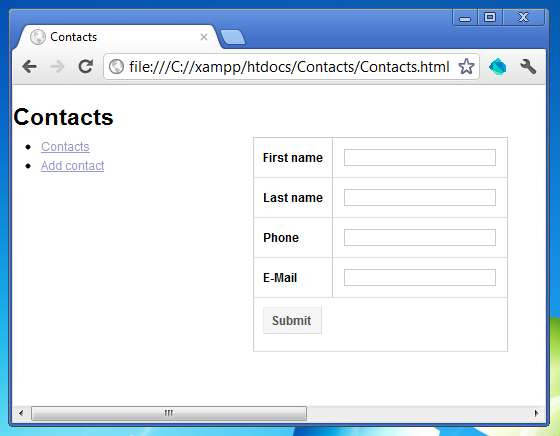
\includegraphics[width=0.8\textwidth]{images/add_view.png}
	\caption{Form for adding a new contact}
	\label{figure:view-1}
\end{figure}

\subsubsection{Listing contacts}

The remaining view will list all contacts using an unordered list (\lstinline[language=HTML]|<ul>|) -- see Listing \ref{listing:view-4}.

\begin{lstlisting}[language=Java,caption={Listing all contacts}\label{listing:view-4}]
// List all contacts view.
class View_List {
  Element element;
  
  View_List(List<Model_Contact> contacts) {
    this.element = new Element.tag('ul');
    
    for (Model_Contact contact in contacts)
    {
      // See the usage of getters and setters:
      this.element.nodes.add(new Element.html('<li>${contact.last_name}, ${contact.first_name} - ${contact.phone} - ${contact.email}</li>'));
    }
  }
}
\end{lstlisting}

\begin{itemize}
\item The constructor expects a list of contact models to build the view.
\item Dart supports a foreach loop to iterate over all elements of the list.
\item For each contact an \lstinline[language=HTML]|<li>| element is added containing last and first name of the contact.
\end{itemize}

\subsection{Controller}

To get access to the views and the model we have to import their libraries:

\begin{lstlisting}[caption={Importing views and model}\label{listing:controller-1}]
// Import views.
#import('View.dart');

// Import model.
#import('Model.dart');
\end{lstlisting}

\begin{itemize}
\item The \lstinline|#import| declarative expects the relative path to the libraries.
\end{itemize}

The \lstinline|run()| method of the contacts controller will make initialization and set up all event handlers of the navigation which will be hard coded.

\begin{lstlisting}[caption={Controller initialization -- the run() method}\label{listing:controller-1}]
// Will do all the initialization
// and set up all needed event handlers.
void run() {

  // A good example for event handling.
  // Will bind the navigation action to the appropriate event handler.
  // For querying CSS selectors are used.
  document.query('#list').on.click.add(list_handler);
  document.query('#add').on.click.add(add_handler);
}
\end{lstlisting}

\begin{itemize}
\item Adding and removing event handlers is done by using the \lstinline|add()| or \lstinline|remove()| method on the chosen event -- here \lstinline|on.click|.
\end{itemize}

% Before looking at the event handlers itself we have to include all views and the used model. Remember we splitted up the application to demonstrate Dart's support for libraries. We declared a ``view'' and a ``model'' library. Now it is time to include them in the main application file:

\subsubsection{Adding a contact}

So let's set up the event handler for adding a new contact -- Listing \ref{listing:controller-3}.

\begin{lstlisting}[caption={\lstinline|add_handler| event handler}\label{listing:controller-3}]
// Event handler for adding a new contact.
var add_handler = (Event event) {
      
  // Prevent default action of link similar to JQuery.
  event.preventDefault();
      
  View_Add view = new View_Add();
      
  // Clean content area before appending the list:
  document.query('#content').nodes.clear(); // Equivalent to JQuery's empty().
  document.query('#content').nodes.add(view.element); // Equivalent to JQuery's append().
      
  // Bind submit event (no real on.submit but on.click).
  document.query('#submit').on.click.add((event) {
    
    Model.add(new Model_Contact.values({
      'first_name': document.query('input#first_name').value,
      'last_name': document.query('input#last_name').value,
      'phone': document.query('input#phone').value,
      'email': document.query('input#email').value,
    }));
  });
};
\end{lstlisting}

\begin{itemize}
\item Similar to JQuery \lstinline|event.preventDefault()| prevents the default action of being executed -- here changing the location due to the link clicked.
\item Then the view is initialized. The content is cleared using \lstinline|nodes.clear()| and the view element is appended.
\item For adding the new contact an event listener \lstinline|on.click| is set, so Dart can handle the form submission and add the new contact using \lstinline|Model.add(Model_Contact contact)|.
\item The value of an input field is accessible through \lstinline|field.value|.
\end{itemize}

%Additionally to just adding the contact we want the user to get feedback -- the user should see a message saying the contact was added successfully instead of leaving the form as it is -- see listing \ref{listing:controller-3}.
%
%\begin{lstlisting}[caption={Give feedback}\label{listing:controller-4}]
%// Clear content.
%// Add success message.
%document.query('#content').nodes.clear();
%document.query('#content').nodes.add(new Element.html('<div class="success">Successfully added contact.</div>'));
%\end{lstlisting}
%
%\begin{itemize}
%\item Clear the content using \lstinline|nodes.clear()| and append the success message.
%\end{itemize}
%
%So the user will get a visually nice feedback:
%
%\begin{figure}[htb]
%	\centering
%  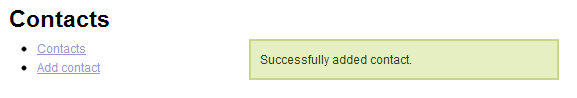
\includegraphics[width=0.9\textwidth]{images/contact_added.png}
%	\caption{``Successfully added contact'' -- nice feedback for the user}
%	\label{figure:view-2}
%\end{figure}

\subsubsection{Listing contacts}

Now have a look at Listing \ref{listing:controller-5} -- the event handler for listing all contacts.

\begin{lstlisting}[caption={\lstinline|list_handler| event handler}\label{listing:controller-5}]
// Event handler for listing all contacts.
var list_handler = (Event event) {
      
  // Prevent default action of link similar to JQuery.
  event.preventDefault();
    
  // Get all contacts.
  List<Model_Contact> contacts = Model.find_all();
      
  View_List view = new View_List(contacts);
      
  // Clean content area before appending the list:
  document.query('#content').nodes.clear(); // Equivalent to JQuery's empty().
      
  // Now add new list of contacts.
  document.query('#content').nodes.add(view.element); // Equivalent to JQuery's append().
};
\end{lstlisting}

\begin{itemize}
\item First the handler gets all contacts through \lstinline|Model.find_all()|.
\item Equivalent to the other view the content is cleared and the view appended to the content.
\end{itemize}

\subsection{Result}

The result could be described as responsive web application. The syntax and a few features of Dart could be shown and will give a brief overview of Dart's capabilities. Nevertheless it is worth having a look at the complete Dart language tour\footnote{\url{http://www.dartlang.org/docs/language-tour/}} and find out more about Dart.

% The contact manager is a good example of Dart's features for working with the DOM and with collections. We created and imported libraries to keep the application as modular as possible. Object-orientation, constructors, private and public attributes were used. Dart offers a lot of possibilities for developing great web applications in a comfortable way.

% Nevertheless there are a lot of features not covered in this paper. So it is worth having a look at the complete Dart language tour\footnote{\url{http://www.dartlang.org/docs/language-tour/}} and find out more about Dart.